\documentclass[a4paper, 11pt, oneside]{report}
\usepackage[utf8]{inputenc}
\usepackage[hmargin=4cm,vmargin=3.5cm,bmargin=3.5cm]{geometry}
\usepackage[portuguese, english]{babel}
\usepackage{graphicx}
\usepackage{hyperref}
\usepackage{helvet}
\usepackage{setspace}
\usepackage{indentfirst}
\usepackage{acronym}

\setlength{\parskip}{0.5cm}
\onehalfspacing

\begin{document}

\def\titulo{Projeto Final}
\def\data{Aveiro, julho 2022}
\def\autores{Pedro Ferreira, João Gaspar, Guilherme Santos, Beatriz Oliveira}
\def\autorescontactos{(98620) \href{mailto:pedrodsf@ua.pt}{pedrodsf@ua.pt}, (107708) \href{mailto:j.gaspar@ua.pt}{j.gaspar@ua.pt},\\(107961) \href{mailto:gssantos@ua.pt}{gssantos@ua.pt}, (108606) \href{mailto:beatrizroliveira@ua.pt}{beatrizroliveira@ua.pt}}
\def\codeua{\textbf{CodeUA:} \url{https://code.ua.pt/projects/labi2022g10}}
\def\departamento{DETI}
\def\empresa{UNIVERSIDADE DE AVEIRO}
\def\logotipo{ua.pdf}

\begin{titlepage}
\begin{center}
\vspace*{50mm}
{\Huge \titulo}\\ 
\vspace{10mm}
{\Large \empresa}\\
\vspace{10mm}
{\LARGE \autores}\\ 
\vspace{30mm}
\begin{figure}[h]
\center
\includegraphics{\logotipo}
\end{figure}
\vspace{30mm}
\end{center}
\end{titlepage}

\title{
{\Huge\textbf{\titulo}}\\
{\Large \departamento\\ \empresa}
}
\author{
\autores \\
\autorescontactos \\\\
\codeua
}
\date{\data}
\maketitle

\pagenumbering{roman}

\selectlanguage{portuguese}

\clearpage

\begin{abstract}
\paragraph{} Este relatório consiste na descrição do enquadramento das tecnologias usadas, na descrição da implementação efetuada, na apresentação de provas que demonstram o seu funcionamento correto, na análise à estrutura da aplicação e nas conclusões finais sobre a solução implementada.\\
\indent Ao longo do relatório, é analisado e explicado o código do programa e do
website que o acompanha, expondo todas as funções e características do projecto.
Após isto, é efectuada uma demonstração do funcionamento do programa
e do modo correto de interacção com a interface do mesmo e o relatório é concluído
com algumas reflexões sobre o projeto e o contributo que este teve para
o desenvolvimento das nossas capacidades. O repositório utilizado para o desenvolvimento da aplicação está alojado no CodeUA e o seu nome é "labi2022g10".
\end{abstract}

\renewcommand{\abstractname}{Agradecimentos}
\begin{abstract}
\paragraph{} Durante a realização deste projeto obtivemos ajudas diretas e indiretas de várias pessoas, assim sendo gostariamos de expressar o nosso enorme agradecimento. Aproveitamos para agradecer ao \textbf{Professor Doutor António Manuel Adrego da Rocha} e ao \textbf{Professor Doutor Diogo Nuno Pereira Gomes}  por nos terem proprocionado as bases necessárias para realizar este projeto (disponibilização de PowerPoints e Guiões que envolvem a matéria).
\end{abstract}

\tableofcontents
\clearpage
\pagenumbering{arabic}

\chapter{Introdução}

\paragraph{} O objetivo deste projeto é desenvolver uma aplicação \textit{Web Online} que armazena e visualiza imagens originais de forma segura e que faz o acompanhamento das transações digitais entre os colecionadores. A aplicação principal tem como módulo principal o \textit{Cherrypy}, que responde corretamente aos pedidos realizados pelo utilizador da aplicação.\\
\indent O relatório está dividido em 5 capítulos. Depois deste Capítulo 1 (Introdução), encontra-se o Capítulo 2 (Desenvolvimento) onde é apresentado e explicado o código que foi desenvolvido. No Capítulo 3 (Resultados) é demonstrado o funcionamento do programa e no Capítulo 4 apresentam-se as conclusões do projeto. Para acabar, é comentada a divisão do trabalho entre os elementos do grupo no Capítulo 5.

\clearpage

\chapter{Desenvolvimento}

\section{Python}

\subsection{Módulos}
\paragraph{} Os módulos usados foram os seguintes:
\begin{itemize}
	\item os.path: obtenção de informações sobre diretórios;
	\item cherrypy: usado para o desenvolvimento da aplicação;
	\item random e string: ambos usados para gerar os tokens, uma string de 16 caracteres \acs{ascii} aleatórios;
	\item sqlite3: usado para operações relacionadas com a base de dados (incluindo criação e métodos);
	\item json: funções de retorno de informação e para obtenção da mesma.
\end{itemize}

\indent O programa começa com a definição de um dicionário que contribui para a configuração da aplicação (\autoref{fig:config}).

\begin{figure}[h]
\center
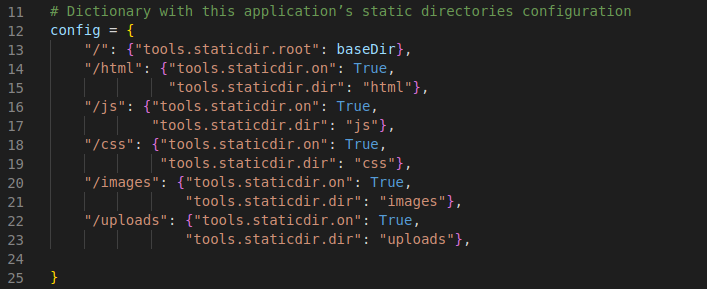
\includegraphics[width=320pt]{configDIC.png}
\caption{Dicionário que contribui para a configuração da aplicação}
\label{fig:config}
\end{figure}

\subsection{Base de Dados}
\paragraph{} Como podemos verificar na figura abaixo (\autoref{fig:create}), toda a função (\textit{def create(sel, username, password):}) é usada para a criação da tabela, caso não exista, será criada uma. A tabela guarda informações como: o nome de utilizador e a password.

\begin{figure}[h]
\center
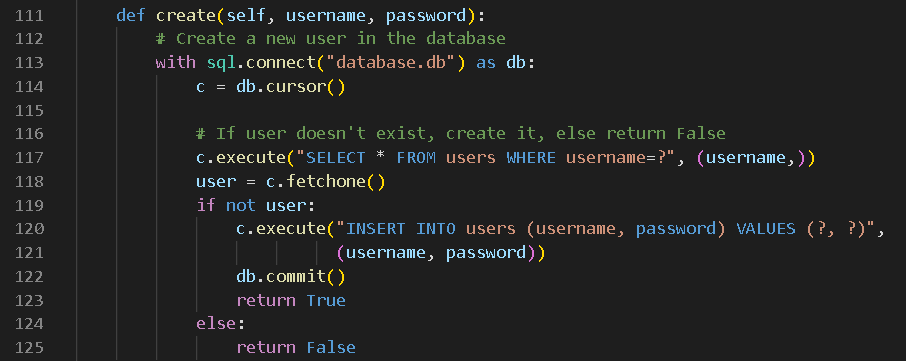
\includegraphics[width=320pt]{createDB.png}
\caption{Criação da base de dados}
\label{fig:create}
\end{figure}

\indent Na \autoref{fig:delete} a função \textit{delete} remove um utilizador da base de dados e a função delete\textunderscore token remove o token do utilizador.

\begin{figure}[h]
    \center
    a) 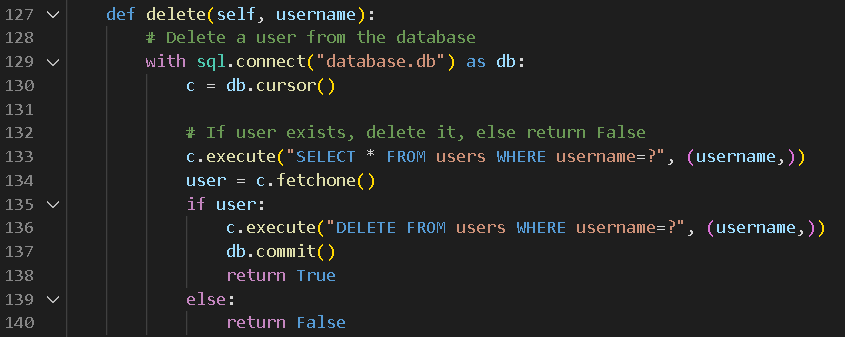
\includegraphics[width=300pt]{deleteDB.png} \\
    b) 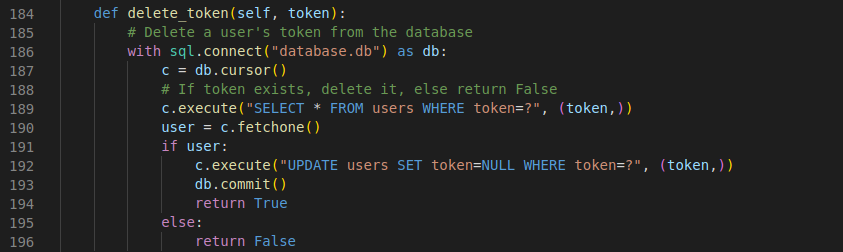
\includegraphics[width=300pt]{deletetokenDB.png}
    \caption{a) Remoção do utilizador da base de dados; b) Remoção do token de utilizador da base de dados.}
    \label{fig:delete}
\end{figure}

\newpage

\indent Na \autoref{fig:valid} a função \textit{valid} "checa" se o token está na base de dados.

\begin{figure}[h]
\center
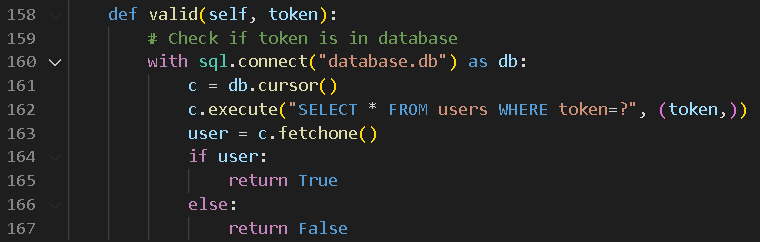
\includegraphics[width=320pt]{validDB.png}
\caption{Validação do token}
\label{fig:valid}
\end{figure}

\indent Por fim a \autoref{fig:auth} refere-se à função \textit{auth} que, caso o utilizador e a password estejam corretas cria um token \textit{\ac{ascii}}.

\newpage

\begin{figure}[h]
\center
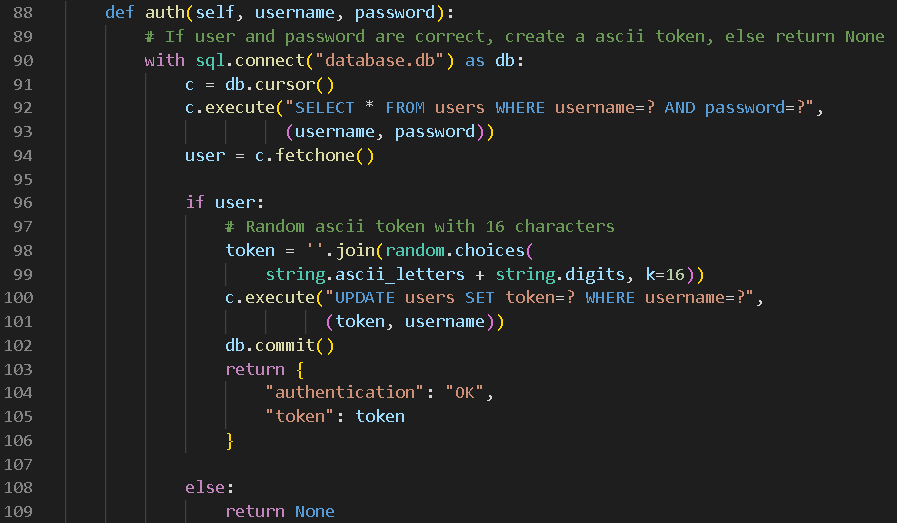
\includegraphics[width=320pt]{authDB.png}
\caption{Criação do um token \ac{ascii}}
\label{fig:auth}
\end{figure}

\subsection{Interligação das Páginas}

\paragraph{} Posteriormente passámos à interligação das páginas que constituíam a interface da aplicação. 

\begin{figure}[h]
\center
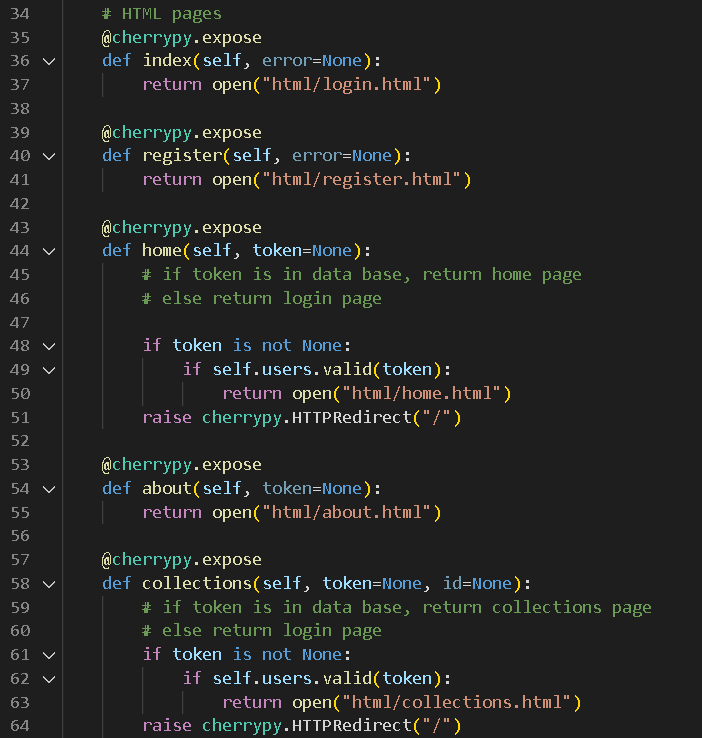
\includegraphics[width=170pt]{htmlPAGE1.png} \\
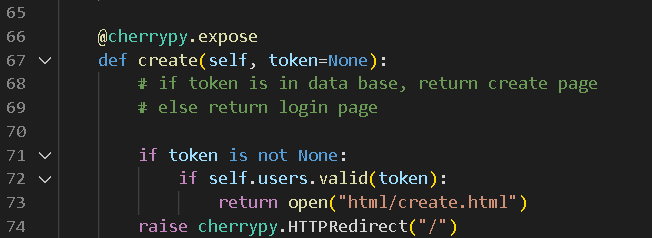
\includegraphics[width=170pt]{htmlPAGE2.png}
\caption{Interligação das páginas}
\end{figure}

\subsection{Sign in, Sign out e Sign up}

\paragraph{} Nesta subseção veremos as funções \textit{sign\textunderscore in}, \textit{sign\textunderscore out} e \textit{sign\textunderscore up} que servem, respetivamente para fazer o login na página \textit{login.html}, para fazer o logout e para fazer um registo novo de utilizador.

\begin{figure}[h]
\center
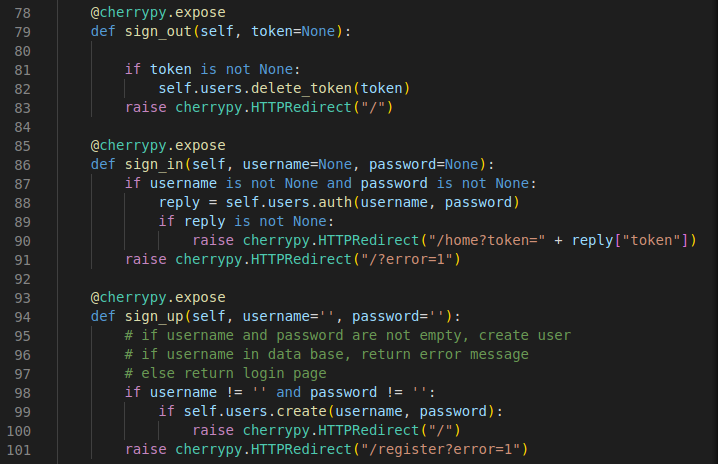
\includegraphics[width=320pt]{signsINOUTUP.png}
\caption{Funções sign's}
\end{figure}

\subsection{Coleções e uploads}

\paragraph{} A figura abaixo (\autoref{fig:colup}) representa duas funções, uma relativa à criação de uma nova coleção (\textit{new\textunderscore collection}) e outra ao upload das imagens de cada utilizador (\textit{upload}).

\begin{figure}[h]
\center
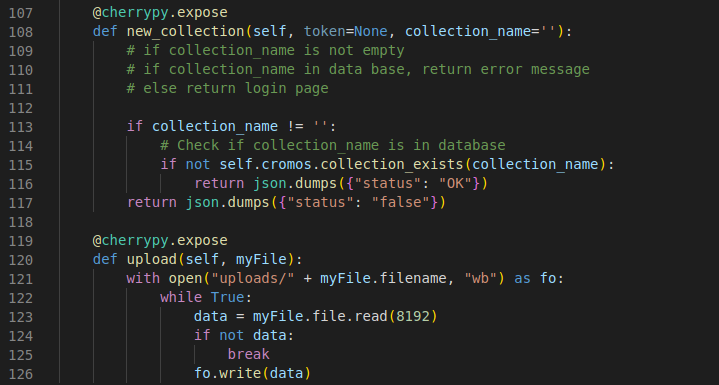
\includegraphics[width=250pt]{colupIMAGE.png}
\caption{Funções criadoras de coleções e upload de imagens}
\label{fig:colup}
\end{figure}

\subsection{Configuração e porta TCP}

\paragraph{} Finalizando esta seção temos na \autoref{fig:port} uma configuração da aplicação e da porta \ac{tcp} usada.

\begin{figure}[h]
\center

\includegraphics[width=320pt]{configPORT.png}
\caption{Configuração da porta}
\label{fig:port}
\end{figure}

\section{HTML, CSS e JavaScript}

\paragraph{} A interface Web foi implementada para uma versão desktop. Os ficheiros \textit{\*.html} das mesmas podem ser facilmente identificados na pasta \textit{html} no diretório principal. A versão é composta por seis ficheiros do tipo \ac{html}, nomeadamente: \textit{login.html}, \textit{register.html}, \textit{home.html}, \textit{collection.html}, \textit{create.html} e \textit{about.html}. Cada um destes ficheiros representa uma página com um propósito específico de interação com o utilizador.\\
\indent Vejamos a implementação da página \textit{home.html} e serão comentadas as seguintes páginas apenas nas suas variações. \\
\indent O head da página \textit{home.html} é "parecido" ao das restantes. Aqui se apresenta o seu código:

\begin{figure}[h]
\center
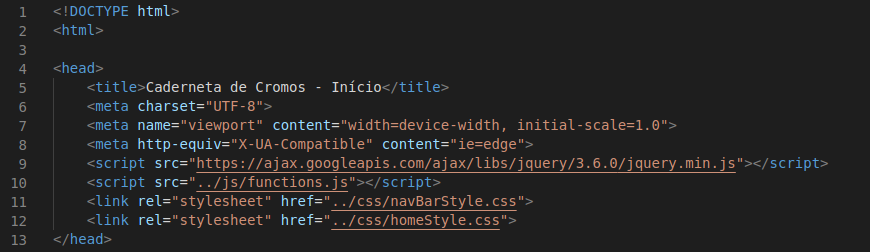
\includegraphics[width=350pt]{headHOME.png}
\caption{HEAD da página \textit{home.html}}
\label{fig:head}
\end{figure}

\indent Tal como se pode observar, as primeiras linhas destinam-se a definir os dados \textit{meta}, que poderão ser usados como por exemplo por motores de busca. Define-se também o título, os \textit{links} para os ficheiros \ac{css} e os \textit{script's} (JavaScript).\\
\indent Na construção do website foi implementado uma barra de navegação no topo
da página que permite acesso ao resto do conteúdo. O bloco de navegação:

\begin{figure}[h]
\center
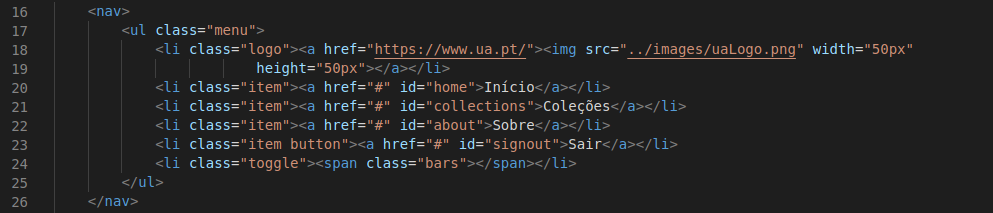
\includegraphics[width=350pt]{navBLOCO.png}
\caption{Bloco de navegação}
\end{figure}

\indent É de notar que o que muda em todas as páginas \acs{html} é precisamente o conteúdo da \autoref{fig:head} e os blocos com os conteúdos das páginas restantes, isto visto o esquema de navegação ser igual em todas exceptuando as páginas \textit{login.html} e \textit{register.html}.\\
\indent A página \textit{login.html}, que se apresenta como página inicial, contém um \textit{head} bastante semelhante ao referido anteriormente, diferindo em pequenos pormenores como os ficheiros \acs{css} e ficheiros que contém os \textit{Scripts} (ou seja, código \textit{JavaScript}) e não apresenta barra de navegação. O mesmo se aplica à página \textit{register.hmtl}.\\
\indent Na página \textit{create.html} o seu conteúdo encontra-se a cargo do JavaScript, sendo que este recebe as imagens inseridas pelo utilizador.\\
\indent A página \textit{collections.html} tem como objetivo disponibilizar as imagens relativas à adição feita na página anteriormente referida.\\
\indent Por último, a página \textit{about.hmtl} disponibiliza ao utilizador informações como os desenvolvedores da aplicação, um mapa com a identificação do DETI, a possibilidade de contactar cada um por e-mail e um pequeno texto informativo.

\clearpage

\chapter{Resultados}

\paragraph{} Na \autoref{fig:inicial} podemos ver uma apresentação da página inicial da aplicação web desenvolvida, onde se pode fazer login ou então registo de utilizador.

\begin{figure}[h]
\center

\includegraphics[width=320pt]{inicioPAGE.png}
\caption{Página inicial}
\label{fig:inicial}
\end{figure}

\indent Se selecionarmos "Não possui conta?" abrirá a página relativa ao registo de novos utilizadores e se posteriormente fizermos \textit{login} passaremos à página principal (\textit{home.html}). Já nesta página o utilizador poderá ver as coleções (ou explorá-las por nome) ou então criar uma coleção, o que o levará à página \textit{create.html}. A partir desta página é possível enviar uma imagem nova, sendo para esse efeito apenas necessário carregar no botão "Explorar..." e escolher a imagem a inserir na coleção.

\newpage

\begin{figure}[h]
\center
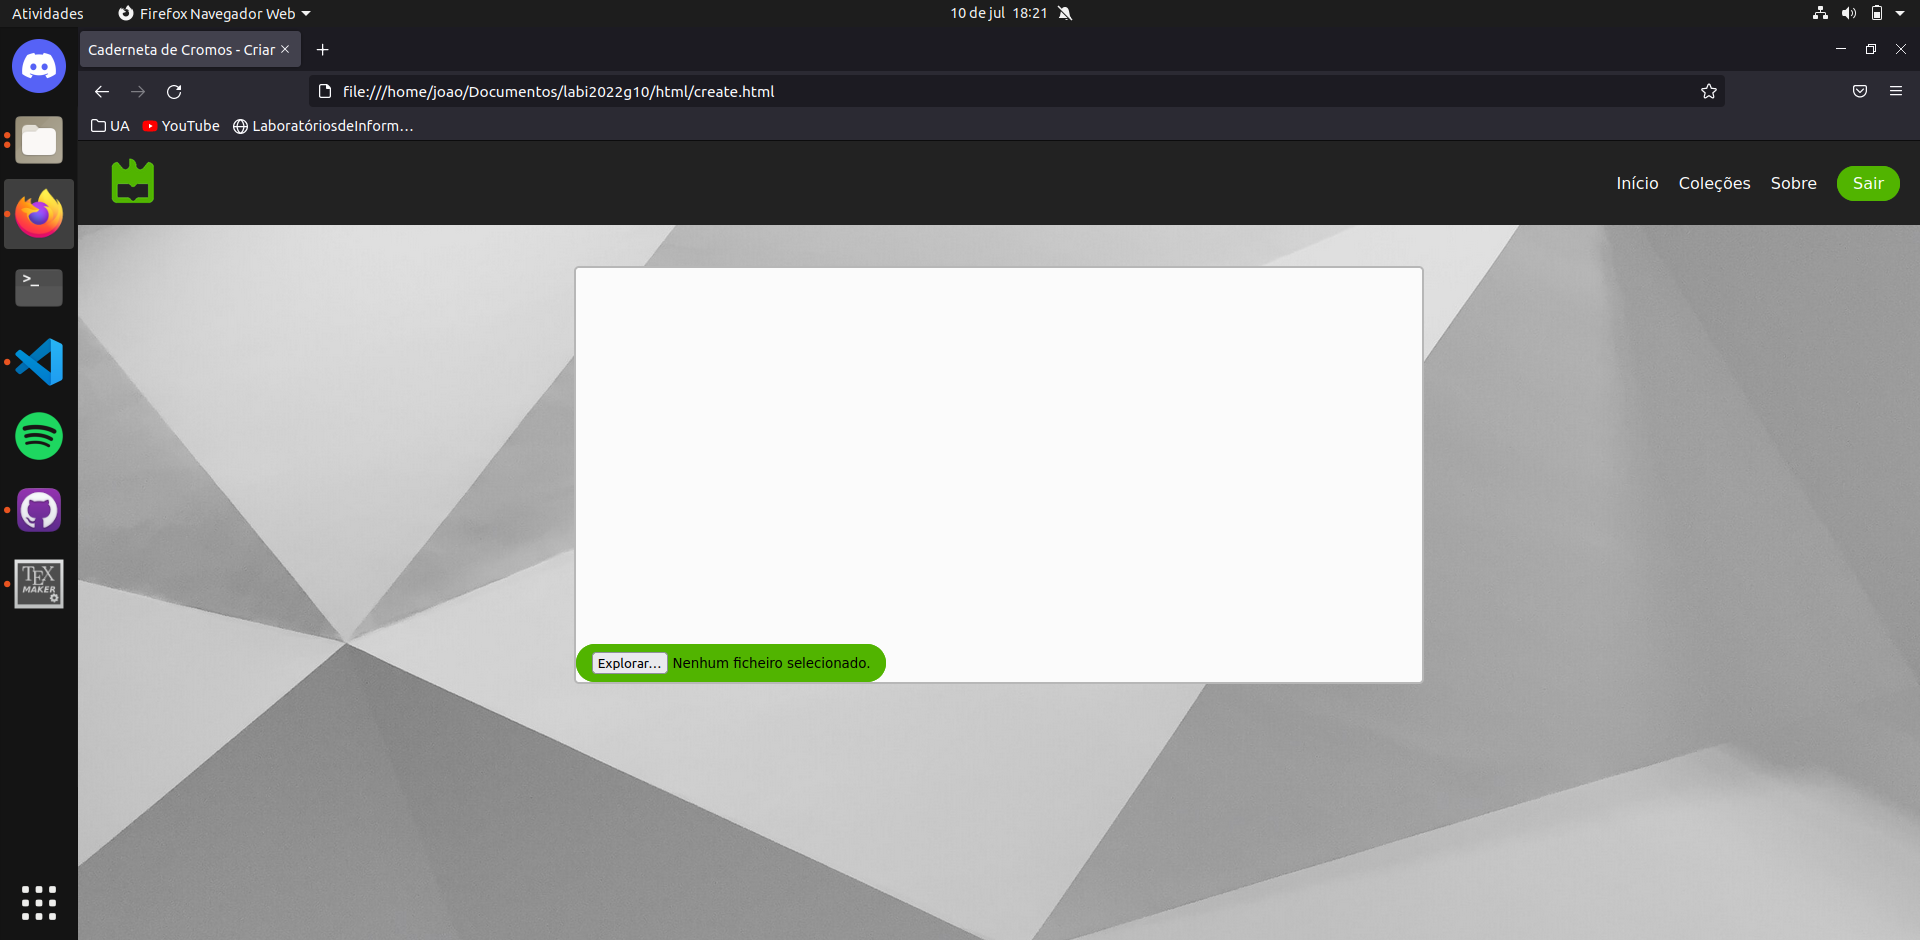
\includegraphics[width=320pt]{createPAGE.png}
\caption{Página \textit{create}}
\end{figure}

\indent Após isso a imagem é apresentada e enviada automaticamente para uma pasta, \textit{uploads}, onde ficará guardada. Quando a coleção estiver de acordo com o pretendido do utilizador, o mesmo poderá, na aba de navegação, percorrer até à página \textit{Coleções} e ver as imagens enviadas.

\section{Objetivos não cumpridos}

\paragraph{} Não foi possível implementar todas as funcionalidades pedidas tal como o processador de imagens cujo objetivo seria lidar com as imagens enviadas para o sistema e a obtenção das mesmas. Em particular deveria suportar a obtenção de uma ou mais imagens. Também não foi possível usar as cifras e colocar marcas de água nas imagens. Estas "falhas" ocorreram devido à má gestão de tempo.

\clearpage

\chapter{Conclusão}

\paragraph{} Neste projeto foi possível consolidar e melhorar os conhecimentos adquiridos ao longo das aulas deste segundo semestre (SQLite3, \acs{json}, CherryPy), como também rever os conhecimentos do semestre anterior (\acs{html}, \acs{css} e \acs{js}), contribuindo assim para a valorização do nosso percurso académico.\\
\indent Com este projeto conseguimos adquirir competências nas áreas de desenvolvimento de aplicações web, manipulação de imagem e bases de dados, para além das competências de aprendizagem que conseguimos atingir, também desenvolvemos de forma proativa o trabalho em equipa (discussão e aceitação de ideias). Apesar das possíveis dificuldades que enfrentamos, procurámos resolver os nossos problemas de forma autónoma e de forma interdependente dentro do nosso grupo de trabalho. Em trabalhos futuros consideramos importante a melhor gestão do tempo em relação a outras \acs{uc}'s, reconhecemos no entanto que trabalhámos arduamente para o que apresentámos aqui.\\
\indent Concluímos que foi uma experiência que nos enriqueceu a vários níveis para um futuro mercado de trabalho, atualmente para o nosso percurso académico e enquanto pessoas.

\chapter*{Contribuições dos autores}

\paragraph{} A divisão do trabalho foi feita da seguinte forma:\\
\indent \ac{pf} desenvolveu o python e a base de dados presente neste projeto.\\
\indent \ac{gs}, \ac{bo} e \ac{jg} assumiram responsabilidade pelo design e aspecto gráfico da aplicação, tendo discutido e planeado a sua parte em conjunto.\\
\indent É importante referir que apesar desta divisão todo o projecto foi discutido, planeado e estruturado pelos 4 membros. As percentagens representativas do trabalho de cada autor são:

\begin{itemize}
\item \acs{pf} - 35\%
\item \acs{jg} - 21\%
\item \acs{gs} - 23\%
\item \acs{bo} - 21\%
\end{itemize}

\indent O relatório foi escrito pelo \acs{jg} e pela \acs{bo}.\\
\indent Foi usado um repositório na plataforma CodeUA para o qual todos os autores
contribuiu com commits frequentes. O link para esse repositório encontra-se
na página \textit{about.html} da aplicação desenvolvida.

\chapter*{Acrónimos}
\begin{acronym}
\acro{json}[JSON]{JavaScript Object Notation}
\acro{html}[HTML]{HyperText Markup Language}
\acro{ascii}[ASCII]{American Standard Code for Information Interchange}
\acro{tcp}[TCP]{Transmission Control Protocol}
\acro{css}[CSS]{Cascading Style Sheets}
\acro{js}[JS]{JavaScript}
\acro{uc}[UC]{Unidade Curricular}
\acro{pf}[PF]{Pedro Ferreira}
\acro{jg}[JG]{João Gaspar}
\acro{gs}[GS]{Guilherme Santos}
\acro{bo}[BO]{Beatriz Oliveira}
\end{acronym}

\end{document}